\documentclass[11pt]{article}

\usepackage[a4paper, total={6.5in, 9.5in}]{geometry}
%\usepackage[T1]{fontenc}
%\usepackage[utf8]{inputenc}
\usepackage[portuguese]{babel}
\usepackage{graphicx}
%\usepackage{ae,aecompl,aeguill}
%\usepackage{showframe}% just to show page geometry, not needed
\setlength{\parskip}{1mm plus 4mm minus 3mm}

\begin{document}

% ========== Edit your name here
\author{
    Rodrigo Orem\\
    \texttt{8921590}
    \and
    Édio Cerati\\
    \texttt{9762678}
    \and
    Thiago Teixeira\\
    \texttt{10736987}
}

\title{\vspace{-2em}Relatório do EP1 -- Parallel Grep}
\maketitle

A implementação do grep paralelo, usando pthreads, foi feita no modelo
produtor-consumidor. Uma thread percorre os arquivos recursivamente no
diretório especificado e coloca eles numa fila. As threads consumidoras
pegam o arquivo da fila e leem ele uma linha por vez: se a linha der
match no pattern, imprime na saída a linha do arquivo.

A fila usada é uma priority queue, onde a prioridade inversa é o tamanho
do arquivo. Dessa forma, nós damos prioridade para processar primeiro os
arquivos menores. Optamos por essa estratégia porque processar arquivos
grandes logo no começo pode fazer com que a saída imprima menos
resultados no começo. Como os arquivos menores podem ser processados
mais rapidamente, o resultado deles também deve ser exibido mais
rapidamente. Nossa avaliação é que isso resulta numa melhor experiência
para o usuário.

Nosso programa usa no mínimo 3 threads. Como nossa arquitetura
implementa o modelo produtor-consumidor, precisamos de pelo menos duas
threads. Além disso, temos a thread main, que cria as outras threads.
Portanto na nossa implementação, a menor quantidade possível de threads
são três.

Nós limitamos o tamanho da fila em mil itens, porque rodar o pgrep na
raiz do sistema de arquivos poderia fazer com que o programa consumisse
toda a memória disponível do sistema. Dessa forma, mesmo em execuções
grandes, a memória do programa não excede 50MB.

Durante o desenvolvimento, tivemos um problema que pode ser interessante
um breve comentário. Aleatoriamente, em algumas execução, o pgrep dava
segmentation fault. Porém ao rodar com o gdb, nunca dava segmentation
fault, mesmo rodando muitas vezes. Após algumas horas e pesquisas,
descobrimos se tratar de um caso clássico de Heisenbug: depurar um
programa altera algumas condições dele, fazendo com que o bug desapareça
quando tentamos observá-lo. No nosso caso, o gdb fazia com que o
programa rodasse mais devagar, portanto diminuía as chances de ocorrer
race conditions. Conseguimos uma stack trace da execução sem usar o gdb,
através do core dump, obtido executando `ulimit -c unlimited` antes de
rodar o programa. O erro era dentro do push da fila, ou seja, o push na
fila não é atômico. Ao colocar o push numa seção crítica o problema foi
resolvido.

Como podemos ver no gráfico a seguir, obtido no Xcode, o trabalho entre
as threads é bem distribuído.

\begin{figure}[!htb]
    {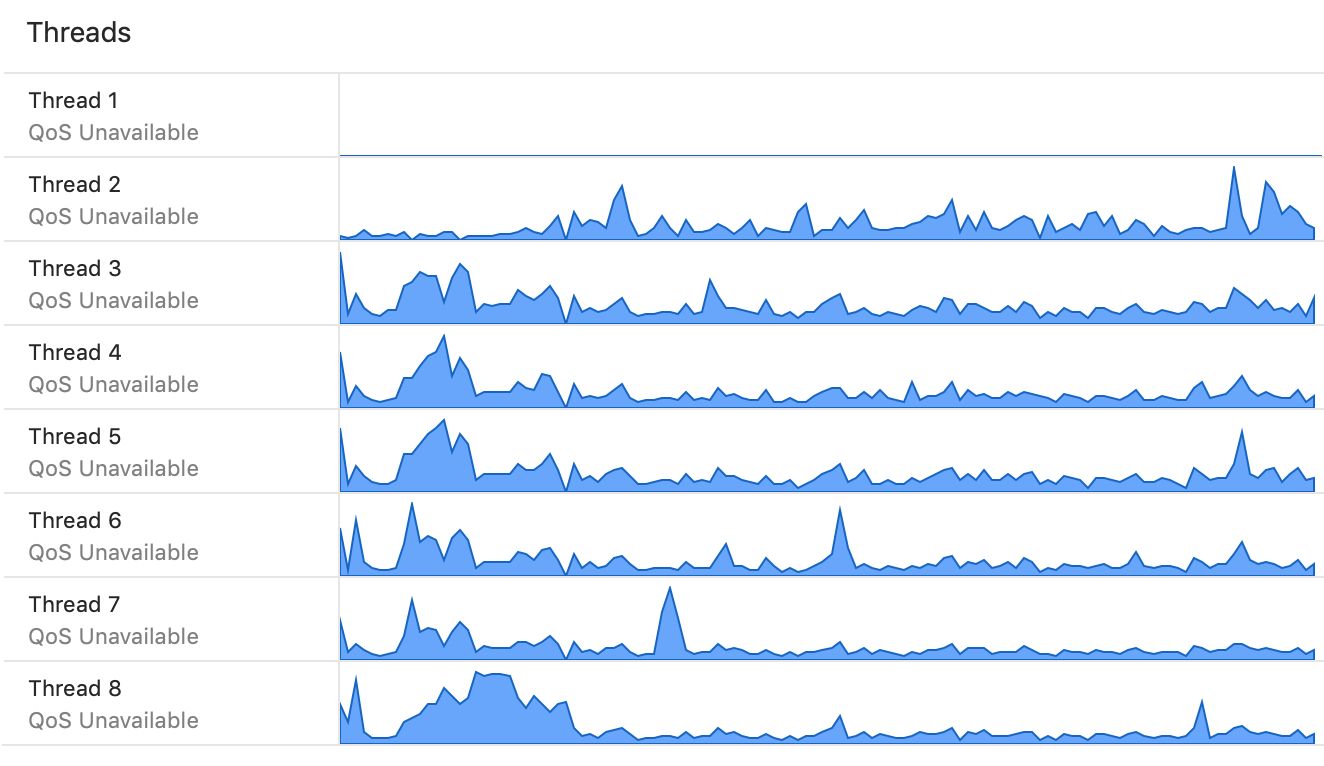
\includegraphics[width=\textwidth]
    {thread-work.png}}
    \caption{\label{fig:thread-work} Trabalho de CPU por thread}
\end{figure}

\end{document}
